\setAuthor{Tundmatu autor}
\setRound{lahtine}
\setYear{2004}
\setNumber{G 10}
\setDifficulty{8}
\setTopic{Staatika}

\prob{Elektriliin}
Elektriülekandeliini postid paiknevad üksteisest $L = \SI{100}{m}$ kaugusel. Postide vahel rippuva traadi keskpunkt paikneb kinnituspunktidest $H = \SI{1}{m}$ võrra madalamal. Traat on valmistatud alumiiniumist, mille tihedus on $\rho = \SI{2700}{kg/m^3}$ ja tõmbetugevus $\SI{100}{MPa}$. Kas traat peab mehaanilisele pingele vastu?

\hint
Ülesande geomeetriat lihtsustab oluliselt $H \ll L$. Lisaks kehtib süsteemis mehaaniline tasakaal. Selle jaoks on mugav vaadelda liini ühe poole jõudude/jõumomendi tasakaalu.

\solu
Leiame pinge traadis. Teatavasti painduvates ahelates mõjub tõmbejõud piki ahela puutujat. Et $H \ll L$, siis traadi kaldenurk on kõikjal väga väike. Jõu horisontaalsihilis komponendi tasakaalust järeldub siis, et pingsus on traadi kõikides punktides praktiliselt ühesugune. Selle jõu mooduli leidmiseks analüüsime näiteks liini parema poole mehaanilist tasakaalu (vt joonist). Kirjutame välja jõumomentide tasakaalutingimus parempoolse kinnituspunkti suhtes:
$$
\frac{m}{2} g \frac{L}{4}=F_{1} H \quad \Rightarrow \quad F_{1}=\frac{m g L}{8 H} .
$$
Siin $m$ on traadi mass. Olgu traadi ristlõige $S$, siis
$$
m=L S \rho \quad \Rightarrow \quad F_{1}=\frac{S g L^{2} \rho}{8 H}
$$
ja pinge traadis
$$
\frac{F_{1}}{S}=\frac{g L^{2} \rho}{8 H} \approx \SI{30}{MPa},
$$
mis ei ületa traadi tõmbetugevust.
\begin{center}
	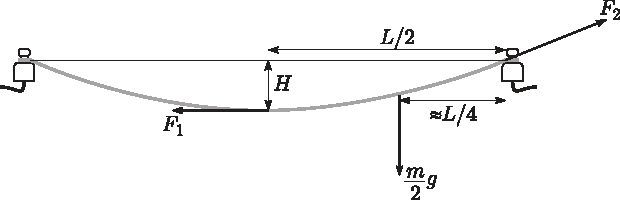
\includegraphics[width=\linewidth]{2004-lahg-10-lah.pdf}
\end{center}
\probend